\documentclass[12pt]{article}
\usepackage{graphicx} %package to manage images
\graphicspath{ {./figures/} }
\usepackage{caption}
\usepackage[font=scriptsize]{subcaption}
\captionsetup[figure]{labelsep=none}
\captionsetup[table]{labelsep=none}
\usepackage{bbm}
\usepackage{amsmath}
\usepackage{import}
\usepackage{array}
\usepackage{booktabs}
\usepackage{afterpage}
\usepackage{floatrow}
\usepackage{pdflscape}
\usepackage{soul}
\usepackage{float}
\usepackage{adjustbox}
\usepackage{longtable}
\usepackage{caption}
\usepackage{setspace}
\usepackage{afterpage}
\usepackage[margin=1in]{geometry}
\usepackage[round]{natbib}
\usepackage{hyperref}
\usepackage{titlesec}

\title{EGC Stata Test 070625 S278}
\author{Sidh Pandit}
\date{August 2025}

\begin{document}

\maketitle

\begin{table}[H]
    \centering
    \scriptsize % shrink text
    \setlength{\tabcolsep}{2pt}
    \renewcommand{\arraystretch}{2}
    \resizebox{\textwidth}{!}{{
\def\sym#1{\ifmmode^{#1}\else\(^{#1}\)\fi}
\begin{tabular}{l*{3}{cccccc}}
\hline\hline
            &\multicolumn{6}{c}{hhinc\_topcoded}                                           &\multicolumn{6}{c}{log\_hhinc\_topcoded}                                       &\multicolumn{6}{c}{log\_hhinc\_topcoded}                                       \\
            &        Mean&          SD&   1st pctl.&      Median&  99th pctl.&         Max&        Mean&          SD&   1st pctl.&      Median&  99th pctl.&         Max&        Mean&          SD&   1st pctl.&      Median&  99th pctl.&         Max\\
\hline
\hline
\(N\)       &        4160&            &            &            &            &            &        3916&            &            &            &            &            &        3584&            &            &            &            &            \\
\hline\hline
\multicolumn{19}{l}{\footnotesize 24-month income is estimated by 24*household income in last 30 days.}\\
\end{tabular}
}
}
    \caption{: Endline raw data summary statistics}
\end{table}


The average per-capita income for households in the sample is \$1.02 a day, which is extreme poverty at the international level. 

There seems to be stark inequality, as for both per-capita and total household income in the last 30 days, the median is almost half of the mean, suggesting a right skewed distribution.


There are large outliers, as seen in the 99th percentile and max values.


\begin{figure}[H]
    \centering
    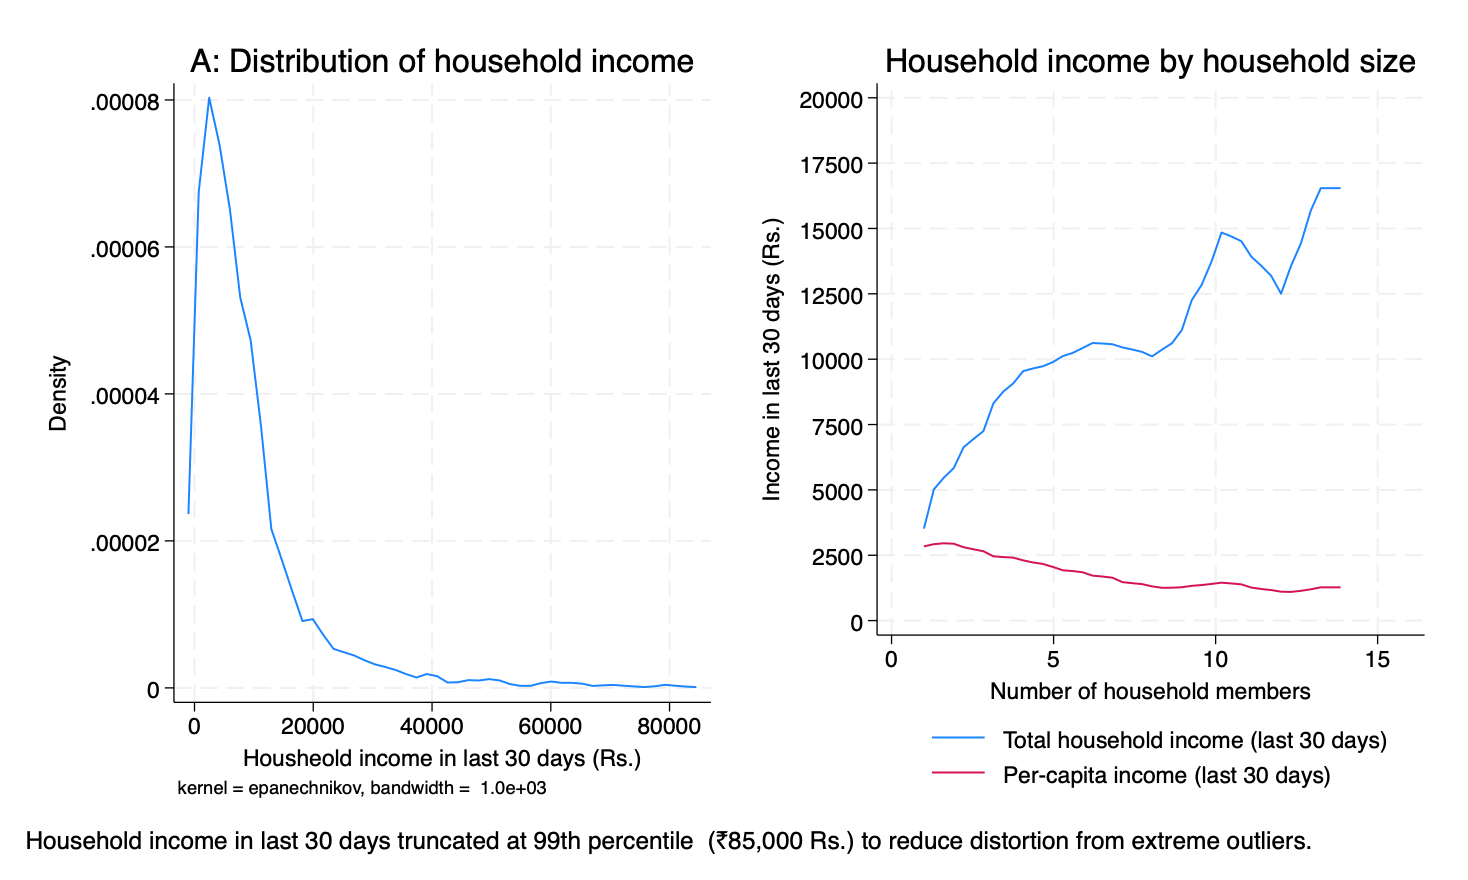
\includegraphics[width=\textwidth]{figures/figure01_hhinc.png}
    \caption{: Distribution and Composition of Household Income in last 30 days}
\end{figure}




\begin{figure}[H]
    \centering
    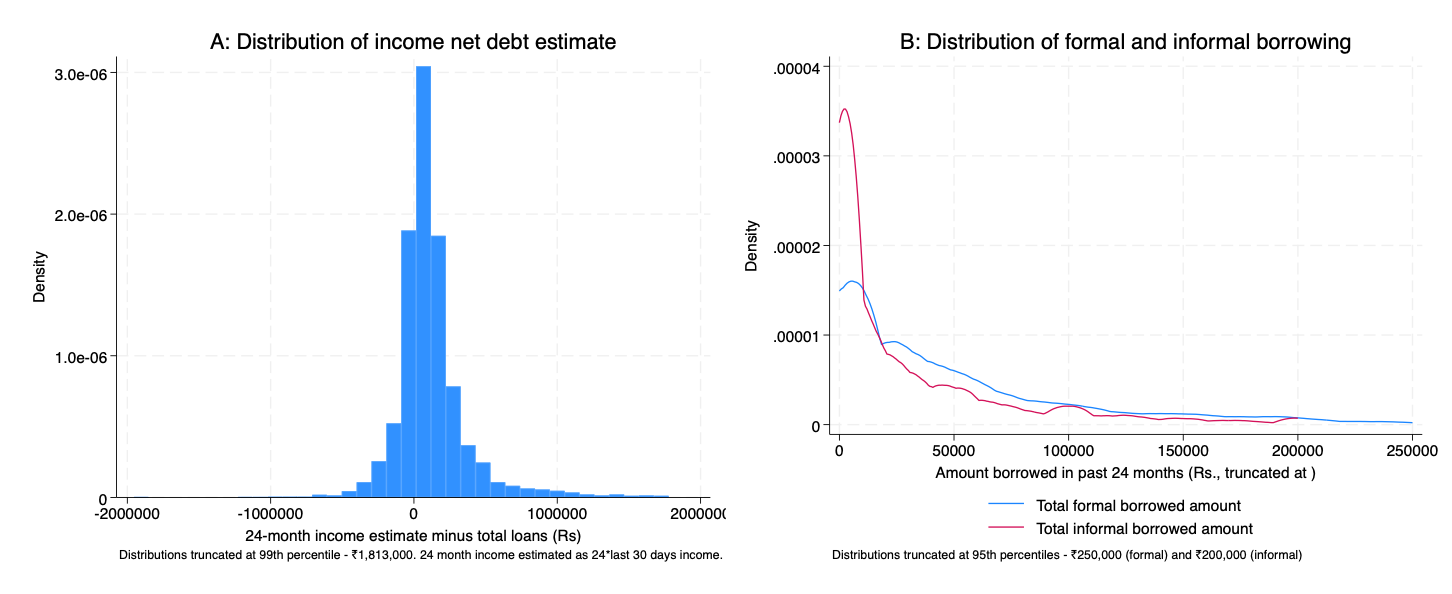
\includegraphics[width=\textwidth]{figures/figure02_loandistribution.png}
    \caption{: Distribution of total borrowing (loans) in last 24 months}
\end{figure}





\section{References used}

\end{document}
